\section{Module: aipy.img}
\label{sec:img}

This imaging module provides functionality for generating images from
visibility data, and for mosaicing images to create maps of the sky.  With
respect to other imaging packages, this one focuses on the providing a
clean and simple imaging solution with native support for correcting
wide-field distortion and projection effects.  Optimizations
such as tapering filters and gridding functions that are intended to
maximize image fidelity without increasing image size in pixels have been
omitted completely en lieu of increasing image size and resolution
to achieve the same effect with some expense in computation.

We will focus on basic imaging and mosaicing machinery in this chapter,
implemented in the Img, ImgW, and SkyHMap classes.  For a more detailed
overview of interferometric imaging, the reader is referred to
``Interferometry and Synthesis in Radio Astronomy, 2nd Edition'' by 
Thompson, Moran, and Swenson \cite{thompson_et_al2001}, and the lecture 
series ``Synthesis Imaging in Radio Astronomy II'' editted by Taylor, Carilli,
and Perley \cite{taylor_et_al1999}.

\subsection{A Brief Introduction}
\label{sec:img_intro}

Synthesis imaging in radio astronomy (the use correlated antennas to 
synthesize a larger, partially filled aperture) relies on inverting
the interferometric measurement equation:

\begin{equation}
V_{\nu}(u,v)=\int\!\!\!\!\int{G_{i,\nu}(\ell,m)G_{j,\nu}^*(\ell,m)
I_\nu(\ell,m)}
{e^{-2\pi i(u\ell+vm+w(\sqrt{\ell^2+m^2}-1))}d\ell dm}
\label{eq:meas_eq}
\end{equation}

This equation relates the frequency-dependent visibilities $V_\nu$ measured by
correlating antennas $i,j$ to the sky brightness $I_\nu$.  Here $ell,m$ are
image coordinates representing $\sin\theta_{EW},\sin\theta{NS}$
respectively.  In the visibility domain, $u,v,w$ represent the seperation
between antennas $i,j$ in equatorial coordinates (EW, radial from pole, NS),
measured in wavelengths. Finally, $G_i, G_j$ remind us that each antenna
can have an independent gain (as a function of frequency and sky position)
that affects the amplitudes and weightings of sources in our measured
visibilities.

The above equation looks a lot like a two-dimensional Fourier transform.  In
fact, if we omit the $w(\sqrt{\ell^2+m^2}-1)$ term, that's exactly what it is.
Forgetting about $w$ for a minute, we should be able to take the {\it inverse}
Fourier transform of our measured visibilities to get an image of the sky.
This can be done efficiently by placing all of our sampled visibilities on a
regularly sampled UV matrix at the appropriate $u,v$ locations (an operation
called ``gridding''), and then using a fast Fourier transform algorithm.  The
problem is that we have incomplete information for inverting this
equation--we've only measured $V_\nu$ at certain $u,v$.  This introduces
predictable effects in our resultant (so-called ``dirty'') image.  If we keep
track of what points we've sampled by placing a real-valued sample weight
(equal to the strength of the sky in the visibility sample we measured) in
a seperate matrix at each $u,v$ point we sample, we can invert this matrix
to get a ``dirty beam'', or a predicted point-spread function representing
what a point source in the center of our image would look like after we
incompletely sample the aperture.  If we deconvolve our dirty image by our
dirty beam, we come up with a ``clean image'', which more closely approximates
what the sky actually looks like.  Various algorithms for deconvolving
are implemented in aipy.deconv.

Deconvolving is imperfect.  We've lost information by not sampling the
whole aperture, so we won't be able to reconstruct a perfect image of the
sky.  It is assumed that for high-quality images, you will have to use
a clean-ed image to predict visibilities for your array, subtract those
predicted visibilities from your measured ones, and then image (and clean)
the residual data to find and correct inaccuracies in you original image.
AIPY contains infrastructure for prediction visibilities from pixel maps,
but this functionality is not yet mature enough for discussion here.

\subsection{Class: Img}

An Img is responsible for storing the UV matrix and the beam matrix that 
can be inverted, using a fast Fourier transform, to get the dirty image
and the dirty beam, respectively.  You start by specifying the size
of your two matrices in UV coordinates by providing a size (number of
wavelengths across your matrix) and a resolution (number of pixels per
wavelength).  The size of your UV matrix determines the resolution
of your image (image resolution = 1 / UV size) and the resolution of
your UV matrix determines the field-of-view of your image on the sky
(image size in $\ell,m$ = 1 / UV resolution):

\subsubsection{A Little About Coordinates}

\begin{verbatim}
>>> import aipy, pylab
>>> im = aipy.img.Img(size=200, res=0.5)
>>> L,M = im.get_LM(center=(200,200))
>>> pylab.subplot(121); pylab.imshow(L); pylab.colorbar(shrink=.7)
>>> pylab.subplot(122); pylab.imshow(M); pylab.colorbar(shrink=.7)
>>> pylab.show()
\end{verbatim}

\begin{figure}
\begin{center}
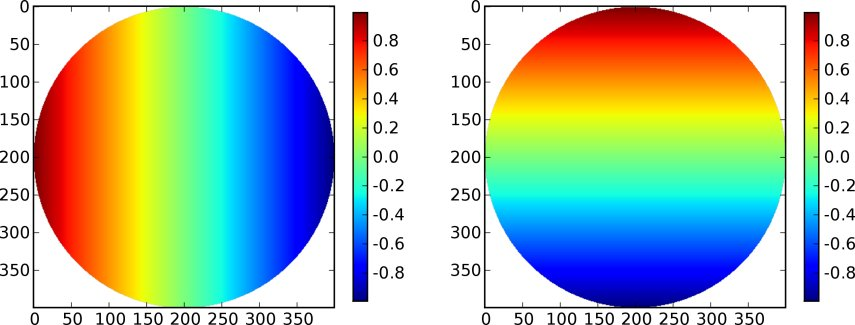
\includegraphics[scale=.4]{img_lm.jpg}
\caption{Plotted are the $\ell,m$ coordinates for an Img with size=200,
res=0.5.  Note that $\ell$ measures +E -W, and $m$ measures +N -S.  AIPY
follows the convention that for images, coordinates increase right to left
and bottom to top (assuming the origin is placed in the top-left corner).  
This presents a geocentric view of the sky.}
\label{fig:img_lm}
\end{center}
\end{figure}

In the above snippet, we've defined a matrix 200 wavelengths across, with a
resolution of 0.5 wavelengths.  In image domain, this generates an image with
a resolution of $\sim0.28^\circ$ near image center (and decreasing resolution
away from center), and a range of $-90^\circ$ to $90^\circ$, since $\ell,m$
range from -1 to 1.  Note that this generates sky coordinates which are
outside the range of physical possibility.  These coordinates are masked,
reading as white in Fig. \ref{fig:img_lm}.  Internally to Img, UV and image
centers are at (0,0).  To recenter for plotting, where it is preferable that
image center is in the middle of the screen, most functions that return a
matrix accept a ``center'' argument with a pixel offset.

AIPY follows the convention that $\ell$ increases right to left, and $m$
increases bottom to top, assuming the origin is placed in the top-left corner
(see Fig. \ref{fig:img_lm}).  This gives us a geocentric view of the sky.
Before we get into actual imaging, lets explore coordinates a little more.
Continuing from above:

\begin{verbatim}
>>> xyz = im.get_top(center=(200,200))
>>> az,alt = aipy.coord.top2azalt(xyz)
>>> pylab.subplot(221); pylab.imshow(az)
>>> pylab.subplot(222); pylab.imshow(alt)
>>> xyz = im.get_eq(ra=0, dec=3.14/4, center=(200,200))
>>> ra,dec = aipy.coord.eq2radec(xyz)
>>> pylab.subplot(223); pylab.imshow(ra)
>>> pylab.subplot(224); pylab.imshow(dec)
>>> pylab.show()
\end{verbatim}

\begin{figure}
\begin{center}
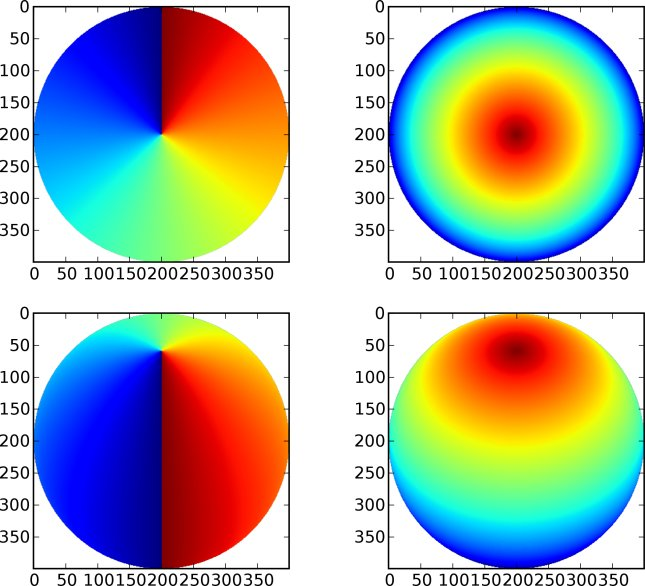
\includegraphics[scale=.4]{img_crd.jpg}
\caption{On the top row are plotted topocentric coordinates for an Img in
azimuth (angle clockwise from N) and altitude (angle from horizon).  The
second row shows right-ascension and declination coordinates in the current
epoch for an observer at $45^\circ$ latitude with 0:00 right ascension
overhead.  Coordinate transformations are provided by the aipy.coord module.}
\label{fig:img_crd}
\end{center}
\end{figure}

The above example (Fig. \ref{fig:img_crd}) illustrates how topocentric
coordinates (useful for calculating beam patterns) and equatorial coordinates
(useful for calculated source positions) at the current epoch are both
available through an Img.  Note that aipy.coord also provides all
functionality for converting between coordinate systems and precessing to
various epochs; the several coordinate systems available through Img are just
for convenience.

\subsubsection{Gridding and Imaging}

It is finally time to generate a dirty image.  To do this, we will gather
visibility samples, calculate the uvw coordinates where they were measured,
and then grid the samples and weights onto a matrix using Img.put().  Finally,
we will use an inverse Fourier transform to generate a dirty image and
matching dirty beam.  For data, we will use the same test.uv file as in
previous sections, with associated parameters recorded in loc.py under
``pwa303''.  This file is attainable via:

\begin{verbatim}
$ wget http://setiathome.berkeley.edu/~aparsons/aipy/test.uv.tar.bz2
$ compress_uv.py -x test.uv.tar.bz2
\end{verbatim}

Starting with a fresh Python interpreter, we will open our Miriad UV file
and prepare an AntennaArray with antenna positions derived from the
``pwa303'' location key in loc.py, and frequency channels matching the
data in the UV file (sdf, sfreq, nchan).  We will also choose a source
(in this case, `vir' indicates Virgo A from src.py) to phase our data to, 
putting it at the center of our image:  

\begin{verbatim}
>>> import aipy, pylab, numpy as n
>>> uv = aipy.miriad.UV('test.uv')
>>> aa = aipy.loc.get_aa('pwa303', uv['sdf'], uv['sfreq'], uv['nchan'])
>>> src = aipy.src.get_src('vir')
\end{verbatim}

Next, we will gather visibility data from the UV file and calculate the
corresponding uvw coordinates using our AntennaArray and celestial source.
We will not include auto-correlation data (uv.select), we will skip 
data where Virgo is below the horizon (the PointingError try-except clause), 
and we will throw out data that is flagged as bad in the data mask 
(the compress/compressed functions).  For more signal-to-noise, we're
including all channels--all data and coordinates are a function of
frequency, making this a multi-frequency map:

\begin{verbatim}
>>> data, uvw, wgts = [], [], []
>>> uv.select('auto', 0, 0, include=False)
>>> for (crd,t,(i,j)),d in uv.all():
>>>     aa.set_jultime(t)
>>>     src.compute(aa)
>>>     try: d, crd = aa.phs2src(d, src, i, j, with_coord=True)
>>>     except(aipy.ant.PointingError): continue
>>>     uvw.append(crd.compress(n.logical_not(d.mask), axis=0))
>>>     data.append(d.compressed())
>>>     wgts.append(n.array([1.] * len(data[-1])))
>>> data,uvw,wgts = n.concatenate(data),n.concatenate(uvw),n.concatenate(wgts)
\end{verbatim}

Note how phs2src() is used now with the with\_coord argument to return the
projected uvw coordinates of a baseline towards the specified source.  The
above also illustrates how different sample weights can be specified for each
data, although in this case we equally weight each sample.  Now that we've
gathered up all our visibility data with uvw coordinate and sample weights,
we are ready to make an image:

\begin{verbatim}
>>> im = aipy.img.Img(size=200, res=.5)
>>> uvw, data, wgts = im.append_hermitian(uvw, data, wgts)
>>> im.put(uvw, data, wgts)
>>> pylab.subplot(221); pylab.imshow(n.abs(im.uv))
>>> pylab.subplot(222); pylab.imshow(n.abs(im.bm))
>>> pylab.subplot(223); pylab.imshow(n.log10(im.image(center=(200,200))))
>>> pylab.subplot(224); pylab.imshow(n.log10(im.bm_image(center=(200,200))))
>>> pylab.show()
\end{verbatim}

\begin{figure}
\begin{center}
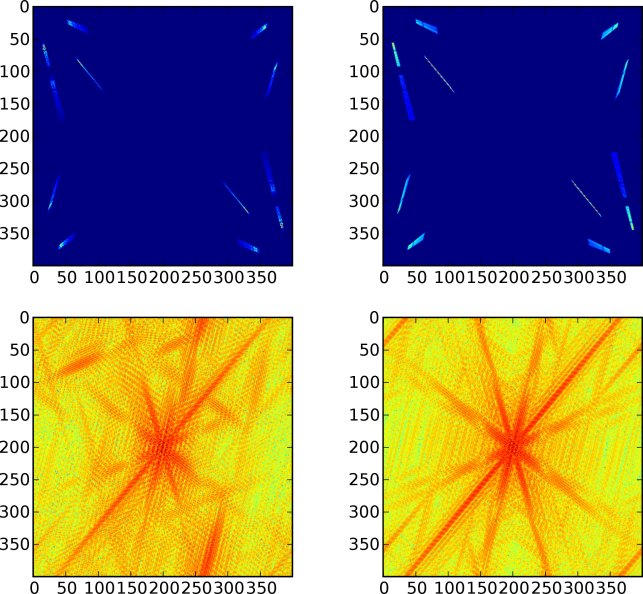
\includegraphics[scale=.4]{img_vir.jpg}
\caption{The upper plots illustrate matrices containing gridded visibility
data (left) and gridded sample weights (right).  Below them are the inverse
Fourier transforms of these matrices, illustrating a dirty image of Virgo A
(left) and the corresponding dirty beam (right).}
\label{fig:img_vir}
\end{center}
\end{figure}

We have specified an Img that is larger than our maximum baseline to be able
to hold all UV data, and we have specifed a resolution that should cover
horizon to horizon.  We used the append\_hermitian() command to generate
the complex-conjugate data at -uvw that complements every (i,j) baseline
with the equivalent (j,i) measurement and ensures that a real-valued sky
image is generated.  Finally, we use put() to grid the data.  Do not
forget that the Img, as opposed to the ImgW presented in the next section,
ignores the w component of each uvw coordinate.

Figure \ref{fig:img_vir} illustrates (left to right, top to bottom) the
UV and beam matrices containing gridded visibility data and sample weights,
respectively, and the dirty image and dirty beam that they generate.
It is reassuring that the source in the center of the image looks basically
like the dirty beam.  The match is not exact because there are other sources
in the image, and because the sample weights we have specified do not exactly
match the weighting of Virgo in the data.  We could have used
the strength of the primary beam in the direction of Virgo as a sample
weight to more closely approximate the dirty beam that will deconvolve
the center of our image.

It is also worth pointing out that the sidelobes of Virgo in our dirty image
wrap around the edges and alias back into our image.  This is an effect
related to the field of view (FoV) of our image, or equivalently, the
resolution of our UV matrix.  Wrapping effects can be combatted by choosing a
resolution corresponding to a larger FoV than we are interested in, or by more
carefully gridding our samples with a convolution kernel that filters near the
edge of the image.  For simplicity, AIPY's Img currently only supports the
former solution.

\subsection{Class: ImgW}

As mentioned in \S\ref{sec:img_intro}, in order to reduce the measurement
equation (Eq. \ref{eq:meas_eq}) to a two-dimensional Fourier transform, we
made an approximation that $w\approx0$.  This approximation introduces an
error that grows in proportion to $\sqrt{\ell^2+m^2}$.  In other words, as
long as we restrict our FoV to a narrow region around phase center where
$\ell,m$ are small, the error introduced by this approximation is small, but
for wide-field imaging (FoV $\buildrel>\over\sim 10^\circ$), image fidelity
deteriorates rapidly from phase center.  Until recently, solutions to the
problem of balancing the algorithmic efficiency of fast Fourier transforms
with wide-field image fidelity were primarily based around faceting images
into multipler phase centers.  In 2003, an elegant algorithm, called W
projection \cite{cornwell_et_al_2003, cornwell_et-al_2005_347}, was introduced
whereby the ``w term'' in the exponential was accounted for as a convolution
allowing one to project a measured visibility back to the $w=0$ plane.  Though
still imperfect as a result of having a partially sampled aperture, this
algorithm more nearly approximates ``correct'' imaging, and results in
point sources remaining coherent farther from phase center than was previously
possible (see Fig. \ref{fig:img_imgw}).

\begin{figure}
\begin{center}
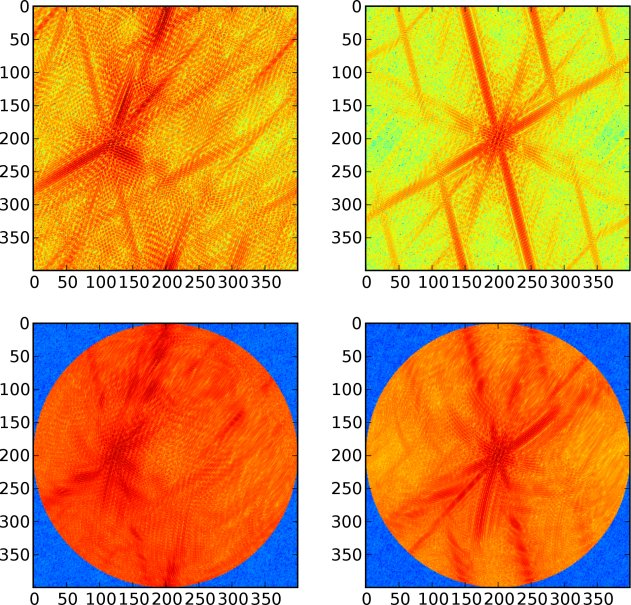
\includegraphics[scale=.4]{img_imgw.jpg}
\caption{The upper plots are the dirty image (left) and dirty beam (right)
generated by an Img phasing 1.5 hours ($22.5^\circ$) from Virgo A, and the 
lower plots illustrate the same using an ImgW.  Notice that the Img fails
to place flux at the actual location of the source, and that the ImgW does
concentrate flux at the source location, but exhibits a point-source response
which departs moderately from the dirty beam.  The convolution inherent to
W projection also helps reduce aliasing.  }
\label{fig:img_imgw}
\end{center}
\end{figure}

The ImgW behaves identically to Img from the user's standpoint, with the
exception that gridding takes longer as a kernel counteracting the effects
of the ``w term'' is convolved with the data after gridding.  To avoid
overly large buffers and to speed the algorithm, uvw samples are gridded
along the w axis with bins proportional to $\sqrt{w}$.  Thus, many samples
can be gridded to a single matrix that is acted upon by a single convolution.
This process occurs every time the put() method is called; to maximize
efficiency, put() should be called as infrequently and with as much data as 
possible.  Beware the other extreme, however, where the buffer of ungridded
visibilities exceeds memory capacity and costly disk accesses ensue.

A final note about sample weights: to correctly reconstruct the dirty beam,
sample weights are convolved by the same W projection kernel as the data.
As a result, the Img.bm matrix can contain complex data.  Furthermore, the
dirty beam is constructed for a source at phase center with sidelobes
extending into the wide field. This illustrates a problem that existed
in the Img, but is made more obvious now--the dirty beam, constructed as
it is from data projected to the phase center, does not necessarily represent
the beam by which sources farther from phase center are convolved.  There
is not an easy a priori way of fixing this.  Most imaging packages include
as part of deconvolution a modelling step whereby components of a dirty
image are used to predict visibilities that are then removed from the
original data, and an image of the residuals is used to iteratively improve
the original image.  AIPY includes both ``pure'' deconvolution for
generic applications, and mechanisms for predicting fringes from pixel
images in order to perform a more accurate deconvolution that accounts for
a changing dirty beam across the image.

\subsection{Class: SkyHMap}

\subsection{Script: plot\_img}
